% Created 2020-07-24 Fri 18:37
% Intended LaTeX compiler: pdflatex
\documentclass[10pt, compress, aspectratio=169, xcolor={table,usenames,dvipsnames}]{beamer}

\usepackage{booktabs}
\mode<beamer>{\usetheme[numbering=fraction, progressbar=none, titleformat=smallcaps, sectionpage=none]{metropolis}}
\usepackage{sourcecodepro}
\usepackage{booktabs}
\usepackage{array}
\usepackage{listings}
\usepackage{multirow}
\usepackage{caption}
\usepackage{xeCJK}
\usepackage{graphicx}
\usepackage[english]{babel}
\usepackage[scale=2]{ccicons}
\usepackage{hyperref}
\usepackage{relsize}
\usepackage{amsmath}
\usepackage{bm}
\usepackage{wasysym}
\usepackage{ragged2e}
\usepackage{textcomp}
\usepackage{pgfplots}
\usepackage{appendixnumberbeamer}
\usepgfplotslibrary{dateplot}
\definecolor{Base}{HTML}{191F26}
\definecolor{Highlight}{HTML}{ffda99}
\definecolor{Accent}{HTML}{bb0300}
\setbeamercolor{alerted text}{fg=Accent}
\setbeamercolor{frametitle}{fg=Base,bg=normal text.bg}
\setbeamercolor{normal text}{bg=black!2,fg=Base}
\setsansfont[BoldFont={Source Sans Pro Semibold},Numbers={OldStyle}]{Source Sans Pro}
\lstdefinelanguage{Julia}%
{morekeywords={abstract,struct,break,case,catch,const,continue,do,else,elseif,%
end,export,false,for,function,immutable,mutable,using,import,importall,if,in,%
macro,module,quote,return,switch,true,try,catch,type,typealias,%
while,<:,+,-,::,/},%
sensitive=true,%
alsoother={$},%
morecomment=[l]\#,%
morecomment=[n]{\#=}{=\#},%
morestring=[s]{"}{"},%
morestring=[m]{'}{'},%
}[keywords,comments,strings]%
\lstdefinelanguage{dockerfile}{
keywords={FROM, RUN, COPY, ADD, ENTRYPOINT, CMD,  ENV, ARG, WORKDIR, EXPOSE, LABEL, USER, VOLUME, STOPSIGNAL, ONBUILD, MAINTAINER},
sensitive=false,
comment=[l]{\#},
morestring=[b]',
morestring=[b]"
}
\lstdefinelanguage{yaml}{
keywords={true,false,null,y,n},
ndkeywords={},
sensitive=false,
comment=[l]{\#},
morecomment=[s]{/*}{*/},
morestring=[b]',
morestring=[b]"
}
\lstset{ %
backgroundcolor={},
basicstyle=\ttfamily\scriptsize,
breakatwhitespace=true,
breaklines=true,
captionpos=n,
commentstyle=\color{Accent},
extendedchars=true,
frame=n,
keywordstyle=\color{Accent},
rulecolor=\color{black},
showspaces=false,
showstringspaces=false,
showtabs=false,
stepnumber=2,
stringstyle=\color{gray},
tabsize=2,
}
\renewcommand*{\UrlFont}{\ttfamily\smaller[3]\relax}
\graphicspath{{../../img/}}
\addtobeamertemplate{block begin}{}{\justifying}
\captionsetup[figure]{labelformat=empty}
\usetheme{default}
\author{ \footnotesize Pedro Bruel, Sitao Huang, Vipin Kumar Kukkala, Sai Rahul Chalamalasetti, Cong Xu, Daniel Dauwe, Darel Emmot, \mbox{Ryan Menhusen}, \mbox{Dejan Milojicic}, \mbox{Alfredo Goldman}}
\date{ \scriptsize July 31, 2020}
\title{Design Space Exploration for High Performance Computing}
\hypersetup{
 pdfauthor={ \footnotesize Pedro Bruel, Sitao Huang, Vipin Kumar Kukkala, Sai Rahul Chalamalasetti, Cong Xu, Daniel Dauwe, Darel Emmot, \mbox{Ryan Menhusen}, \mbox{Dejan Milojicic}, \mbox{Alfredo Goldman}},
 pdftitle={Design Space Exploration for High Performance Computing},
 pdfkeywords={},
 pdfsubject={},
 pdfcreator={Emacs 26.3 (Org mode 9.2.5)},
 pdflang={English}}
\begin{document}

\maketitle

\section{Outline}
\label{sec:org65aa6e0}
\begin{frame}[label={sec:orgc015660}]{Outline}
\begin{enumerate}
\item Design Space Exploration and Autotuning
\item Key Results and Current Work
\begin{itemize}
\item Endpoint Congestion Control
\item Bit Quantization on Deep Neural Network Layers
\end{itemize}
\item Perspective: Design Space Exploration as a Service
\end{enumerate}
\end{frame}
\section{Autotuning}
\label{sec:orga4d0ccd}
\begin{frame}[label={sec:org458b662}]{Optimizing Program Configurations}
\begin{columns}
\begin{column}{0.5\columnwidth}
\begin{block}{Architectures for High Performance Computing}
\begin{center}
\includegraphics[width=\columnwidth]{../../../img/architectures_2.png}
\end{center}

How to write \alert{efficient code} for each of these?

\begin{block}{Autotuning}
\vspace{.2cm}

The process of automatically finding a \mbox{\alert{configuration}} of a program
that optimizes an \mbox{\alert{objective}}
\end{block}
\end{block}
\end{column}

\begin{column}{0.5\columnwidth}
\begin{block}{Configurations}
\begin{itemize}
\item Algorithms
\begin{itemize}
\item Sorting, encoding, \(\dots\)
\end{itemize}
\item Implementations
\begin{itemize}
\item Code transformation, libraries, \(\dots\)
\end{itemize}
\item Context-specific parameters
\begin{itemize}
\item Compilers, kernels, \(\dots\)
\end{itemize}
\end{itemize}

\begin{block}{Objectives}
\begin{itemize}
\item Execution time
\item Resource consumption
\item Binary size
\item \(\dots\)
\end{itemize}
\end{block}
\end{block}
\end{column}
\end{columns}
\end{frame}

\begin{frame}[label={sec:org0a1038d}]{Defining Autotuning Search Spaces}
\begin{columns}
\begin{column}{0.4\columnwidth}
\begin{block}{Search Spaces}
\begin{itemize}
\item \alert{Dimension}: Number of configurable parameters
\item \alert{Size}: Number of possible combinations of parameters, or configurations
\end{itemize}

Represent the \alert{effect} of all possible
configurations on target objectives

Can be difficult to explore, with multiple \mbox{\alert{local optima}}
and \mbox{\alert{undefined}} \mbox{\alert{regions}}
\end{block}
\end{column}

\begin{column}{0.6\columnwidth}
\begin{center}
\includegraphics[width=\columnwidth]{../../../img/seymour2008comparison.pdf}
\end{center}

\begin{center}
\scriptsize{Seymour K. \emph{et al.}, A Comparison of Search Heuristics \\ for Empirical
  Code Optimization (CLUSTER 2008)}
\end{center}
\end{column}
\end{columns}
\end{frame}

\begin{frame}[label={sec:org1e550dc}]{Most Common Autotuning Approaches}
\begin{columns}
\begin{column}{0.5\columnwidth}
\begin{block}{Most Common Approaches}
\footnotesize
\begin{itemize}
\item \colorbox{red!25}{Exhaustive}
\item \colorbox{green!25}{Meta-Heuristics}
\item \colorbox{cyan!25}{Machine Learning}
\end{itemize}
\normalsize
\vspace{-.4cm}
\begin{table}
    \centering
    \begin{tabular}{@{}lll@{}}
        \toprule
        System & Domain & Approach \\ \midrule
        \rowcolor{red!25} ATLAS & Dense Linear Algebra & Exhaustive\\ \addlinespace
        \rowcolor{green!25} INSIEME & Compiler & Genetic Algorithm \\
        \rowcolor{green!25} Active Harmony & Runtime & Nelder-Mead \\
        \rowcolor{green!25} ParamILS & Domain-Agnostic & Stochastic Local Search \\
        \rowcolor{green!25} OPAL & Domain-Agnostic & Direct Search \\
        \rowcolor{green!25} OpenTuner & Domain-Agnostic & Ensemble \\ \addlinespace
        \rowcolor{cyan!25} MILEPOST GCC & Compiler & Machine Learning \\
        \rowcolor{cyan!25} Apollo & GPU kernels & Decision Trees \\ \addlinespace
        \bottomrule
    \end{tabular}
\end{table}

\end{block}
\end{column}

\begin{column}{0.5\columnwidth}
\begin{block}{Core Assumptions}
\begin{itemize}
\item A large number of function evaluations
\item Good solutions are reachable
\item Seach space ``smoothness''
\end{itemize}
\begin{block}{After Optimization}
\begin{itemize}
\item \alert{Learn ``nothing''} about the search space
\item \alert{Can't explain} why optimizations work
\end{itemize}
\end{block}
\begin{block}{We have used}
\begin{itemize}
\item Search Heuristics
\item Statistical Learning
\begin{itemize}
\item Experimental Design
\item Gaussian Process Regression
\end{itemize}
\end{itemize}
\end{block}
\end{block}
\end{column}
\end{columns}
\end{frame}
\section{Key Results and Current Work}
\label{sec:orgfb3c47a}
\begin{frame}[label={sec:orgc184d20}]{Summary of Key Results and Current Work}
\small
\begin{table}[htbp]
\caption{SH: Search Heuristics, ED: Experimental Design, GPR: Gaussian Process Regression}
\centering
\begin{tabular}{p{0.28\columnwidth}p{0.08\columnwidth}p{0.44\columnwidth}}
\toprule
Domain & Method & Key Result\\
\midrule
Endpoint Congestion Control & ED & \emph{Ongoing}: Models with increased accuracy\\
Quantization for DNNs & ED, GPR & \emph{Ongoing}: Up to 2\texttimes{} model size reduction\\
\midrule
StST HPC Kernels for GPUs & ED & Consistently finds the global optimum\\
StST HPC Kernels for CPUs & ED, GPR & Up to 10\texttimes{} speedup with a tight budget\\
HLS for FPGAs & SH & Up to 5\texttimes{} decrease on DSP usage\\
CUDA Compiler & SH & Up to 4\texttimes{} speedup\\
\midrule
PETSc Library &  & \emph{Expected}: Up to 10\texttimes{} speedups\\
Rustc and GCC & \multirow{-2}{*}{ED} & \emph{Expected}: Up to 4\texttimes{} speedups\\
\bottomrule
\end{tabular}
\end{table}
\end{frame}
\begin{frame}[label={sec:org73078e2}]{Autotuning for Endpoint Congestion Control}
\begin{columns}
\begin{column}{0.4\columnwidth}
\begin{center}
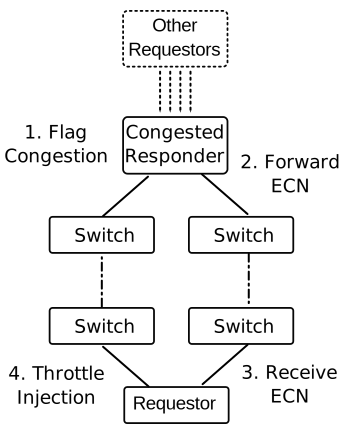
\includegraphics[width=\columnwidth]{../../../img/congestion.pdf}
\end{center}
\end{column}
\begin{column}{0.6\columnwidth}
\begin{block}{Benefits of an Experimental Design Approach}
\vspace{0.8em}

The search  space has  regions of  expressive \alert{measurement  variability}.  Our
approach uses low-discrepancy sampling and quantile regression to:

\begin{itemize}
\item Reduce \alert{simulation costs}
\item Build \alert{statistical models}
\item \colorbox{Highlight}{Increase \alert{prediction accuracy}}
\end{itemize}
\end{block}
\end{column}
\end{columns}
\end{frame}

\begin{frame}[label={sec:orge5fff58}]{A Simplified Congestion Control Problem}
\begin{columns}
\begin{column}{0.5\columnwidth}
\begin{block}{Endpoint Congestion Control}
\begin{itemize}
\item Explicit Congestion Notification
\item Control Injection rates
\end{itemize}
\begin{block}{Search Space Definition}
\begin{center}
\begin{tabular}{ll}
\toprule
Parameter & Value\\
\midrule
Injection Rate 1 & \(inj_1 \in [0.0, 1.0]\)\\
Injection Rate 2 & \(inj_2 \in [0.0, 1.0]\)\\
\bottomrule
\end{tabular}
\end{center}
\end{block}
\end{block}
\end{column}
\begin{column}{0.5\columnwidth}
\begin{block}{Objective}
\begin{itemize}
\item Consider only two adversary applications
\item \alert{Minimize} execution times \(\mathcal{P}_1\) and \(\mathcal{P}_2\), and
\item \alert{Maximize} injection rates \(inj_1\) and \(inj_2\)
\end{itemize}
\begin{block}{Target Performance Metric}
\begin{align*}
  \mathcal{P}(inj_1,inj_2) =
  \; & \dfrac{\mathcal{P}_1(inj_1) + \mathcal{P}_2(inj_2)}{2} + \\
  \; & \left|\left(1  -  \left(\dfrac{inj_1  + inj_2}{2}\right)\right)\right|
\end{align*}
\end{block}
\end{block}
\end{column}
\end{columns}
\end{frame}
\begin{frame}[label={sec:org3382131}]{Injection Rate Search Space}
\begin{columns}
\begin{column}{0.5\columnwidth}
\begin{block}{Unbiased Sample}
\begin{center}
\includegraphics[width=\columnwidth]{../../../img/injection_rates_sobol.pdf}
\end{center}
\end{block}
\end{column}
\begin{column}{0.5\columnwidth}
\begin{block}{Search Space}
\begin{center}
\includegraphics[width=\columnwidth]{../../../img/injection_rates_search_space.pdf}
\end{center}
\end{block}
\end{column}
\end{columns}
\end{frame}
\begin{frame}[label={sec:orgba0b14d}]{Experimental Design for Injection Rates}
\begin{columns}
\begin{column}{0.5\columnwidth}
\begin{block}{Experimental Design: 15 Samples}
\begin{center}
\includegraphics[width=\columnwidth]{../../../img/injection_rates_federov.pdf}
\end{center}
\end{block}
\end{column}
\begin{column}{0.5\columnwidth}
\begin{block}{Performance Prediction}
\begin{center}
\includegraphics[width=\columnwidth]{../../../img/injection_rates_quantile.pdf}
\end{center}
\end{block}
\end{column}
\end{columns}
\end{frame}
\begin{frame}[label={sec:org8305340}]{Experimental Design for a Larger Problem}
\begin{columns}
\begin{column}{0.5\columnwidth}
\begin{block}{Search Space Definition}
\begin{itemize}
\item T\textsubscript{s}: congestion sampling window
\item T\textsubscript{p}: Packet generation delay
\item PIDT\textsubscript{0,31}(T\textsubscript{p}): Throttling table
\item F: ECN flagging threshold
\end{itemize}
\begin{block}{Constraints}
\begin{itemize}
\item T\textsubscript{s} \(\ge\) minimum round-trip time
\item \(PIDT_i < PIDT_{i + 1}\)
\end{itemize}
\end{block}
\end{block}
\end{column}
\begin{column}{0.5\columnwidth}
\begin{block}{Target Performance Metrics}
\begin{itemize}
\item Packet latency
\begin{itemize}
\item Weighted sum of mean and minimum
\item Several applications
\end{itemize}
\item Link bandwidth
\end{itemize}
\begin{block}{Issues with Measurement Time}
\begin{itemize}
\item Experiments are expensive
\item Model-building efforts
\end{itemize}
\end{block}
\end{block}
\end{column}
\end{columns}
\end{frame}

\begin{frame}[label={sec:org61355ae}]{Autotuning DNN Quantization}
\begin{columns}
\begin{column}{0.42\columnwidth}
\begin{center}
\includegraphics[width=\columnwidth]{../../../img/haq_quantization.pdf}
\end{center}

\begin{center}
\scriptsize{HAQ: Hardware-Aware Automated Quantization\\with Mixed Precision (CV 2018)}
\end{center}
\end{column}
\begin{column}{0.58\columnwidth}
\begin{block}{Benefits of an Experimental Design Approach}
\vspace{0.8em}

Our approach uses Gaussian Process  Regression (GPR), and in comparison with
Reinforcement Learning (RL), achieves:

\begin{itemize}
\item More \alert{consistent results}
\item \colorbox{Highlight}{Trade some accuracy for \alert{up to $2\times$ size reduction}}
\end{itemize}
\end{block}
\end{column}
\end{columns}
\end{frame}
\begin{frame}[label={sec:orga364310}]{Autotuning DNN Quantization: ResNet50}
\begin{columns}
\begin{column}{0.5\columnwidth}
\begin{block}{Search Space Definition for ResNet50}
\begin{center}
\begin{tabular}{ll}
\toprule
Parameter & Value\\
\midrule
Bitwidth for Layer 1 & \(q_1 \in [1, 8]\)\\
\(\cdots{}\) & \(\cdots{}\)\\
Bitwidth for Layer 54 & \(q_{54} \in [1, 8]\)\\
\bottomrule
\end{tabular}
\end{center}

\begin{itemize}
\item \(8^{54} \approx\) \alert{\(10^{48}\)} configurations
\item \alert{\(10\) min+} to measure each
\end{itemize}
\end{block}
\end{column}
\begin{column}{0.5\columnwidth}
\begin{block}{Objective}
\begin{itemize}
\item \alert{Minimize} size in MB \(\mathcal{S}\), and
\item \alert{Maximize} Top1 and Top5 accuracy \(\mathcal{A}_{1}\), \(\mathcal{A}_{5}\)
\end{itemize}
\begin{block}{Target Performance Metric}
\begin{align*}
  \mathcal{P}(q_1, \dots, q_{54}) =
  \; & (w_{size}\mathcal{S}(q_1, \dots, q_{54}) + \\
  \; & w_{Top1}\mathcal{A}_1(q_1, \dots, q_{54}) + \\
  \; & w_{Top1}\mathcal{A}_5(q_1, \dots, q_{54})) / \\
  \; & (w_{size} + w_{Top1} + w_{Top5})
\end{align*}
\end{block}
\end{block}
\end{column}
\end{columns}
\end{frame}
\begin{frame}[label={sec:org1cd93c4}]{Gaussian Process Regression for DNN Quantization}
\begin{center}
\includegraphics[width=\columnwidth]{../../../img/gpr_rloriginal_comparison.png}
\end{center}
\end{frame}

\begin{frame}[label={sec:org6b4072f}]{Gaussian Process Regression for DNN Quantization}
\begin{center}
\includegraphics[width=\columnwidth]{../../../img/gpr_rl_comparison.png}
\end{center}
\end{frame}

\section{Design Space Exploration as a Service}
\label{sec:org3b8c54d}
\begin{frame}[label={sec:org94dd3cf}]{Common Design Space Exploration Issues}
\begin{columns}
\begin{column}{0.5\columnwidth}
\begin{block}{Specifying an Autotuning Problem}
\vspace{0.8em}

For each domain, we must determine:

\begin{itemize}
\item Configurable parameters
\item Performance metrics
\item Software dependencies
\item Optimization method
\end{itemize}
\end{block}
\end{column}

\begin{column}{0.5\columnwidth}
\begin{block}{Expected Results}
\vspace{0.8em}

In each domain, we expect to find:

\begin{itemize}
\item Best experiments to run
\item Optimized configuration
\item A useful \alert{statistical model}
\end{itemize}

\begin{block}{Handcrafted Autotuners}
\begin{itemize}
\item Time-consuming
\item Domain-specific problems
\end{itemize}
\end{block}
\end{block}
\end{column}
\end{columns}

\begin{center}
  \colorbox{Highlight}{A \alert{service-based architecture} can encapsulate common solutions,}
  \colorbox{Highlight}{while users focus locally on \alert{domain-specific problems}}
\end{center}
\end{frame}

\begin{frame}[label={sec:orgf84c4b3}]{Design Space Exploration as a Service}
\begin{center}
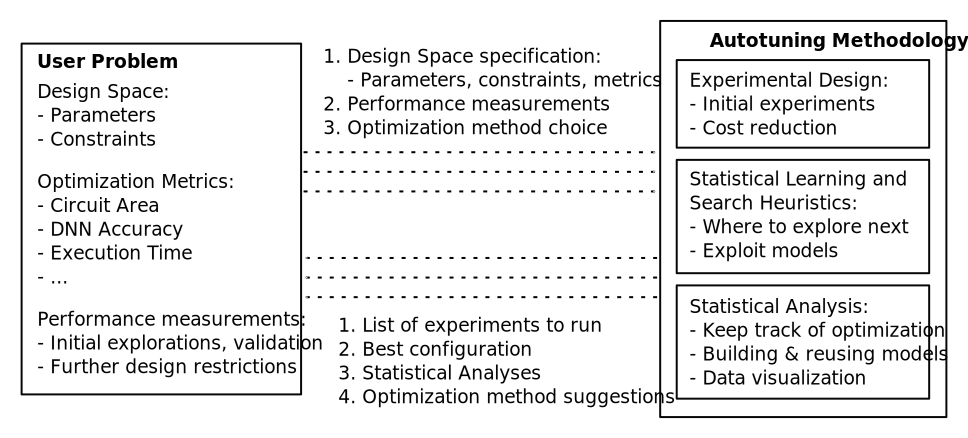
\includegraphics[width=\columnwidth]{../../../img/dse_summary.pdf}
\end{center}
\end{frame}
\begin{frame}[label={sec:org371aae9}]{Design Space Exploration as a Service}
\begin{center}
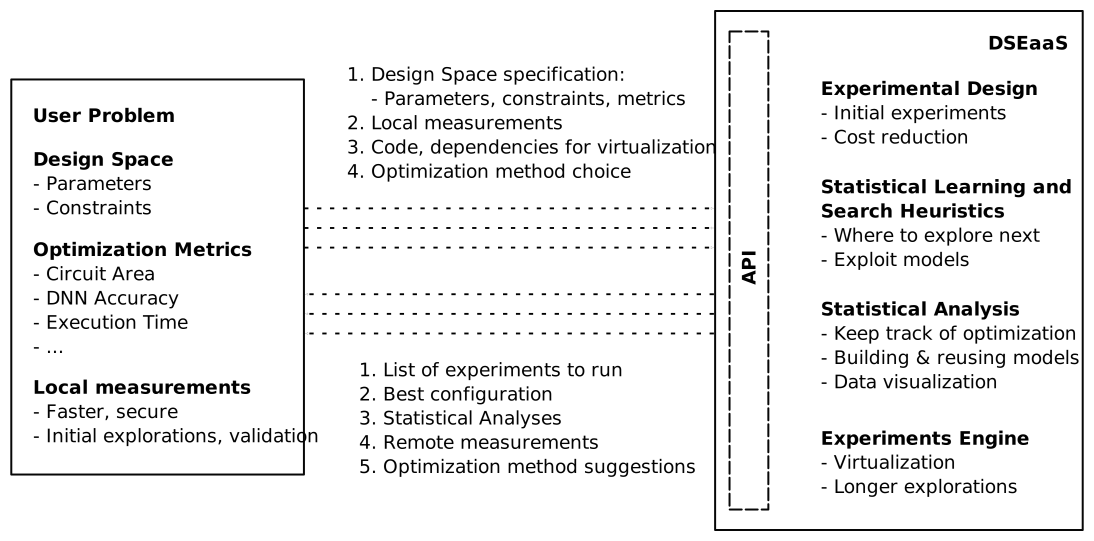
\includegraphics[width=\columnwidth]{../../../img/dseaas_test.pdf}
\end{center}
\end{frame}

\maketitle
\appendix
\begin{frame}[label={sec:orga34e24f}]{Hardware and Performance Trends: The Case for Autotuning}
\begin{columns}
\begin{column}{0.5\columnwidth}
\only<1>{
\begin{figure}[htbp]
\centering
\includegraphics[width=\columnwidth]{../../../img/49_years_processor_data.pdf}
\caption{\url{http://wikipedia.org/wiki/Transistor_count} \url{http://wikipedia.org/wiki/Microprocessor_chronology}}
\end{figure}
}
\only<2>{
\begin{figure}[htbp]
\centering
\includegraphics[width=\columnwidth]{../../../img/top500_rmax_rpeak.pdf}
\caption{\url{https://www.top500.org}}
\end{figure}
}
\end{column}

\begin{column}{0.5\columnwidth}
\begin{block}{Breakdown of Frequency Scaling}
\begin{itemize}
\item Power and temperature constraints
\item Physical limits on frequency
\item Manufacturing processes continue to scale
\end{itemize}

\begin{block}<2>{Sustained Performance Scaling}
\begin{itemize}
\item Multicore, accelerators
\item \colorbox{Highlight}{Software optimization: \alert{Autotuning}}
\end{itemize}
\end{block}
\end{block}
\end{column}
\end{columns}
\end{frame}
\begin{frame}[label={sec:orgd1ebbf4}]{Overview High Dimensional Autotuning Search Spaces}
\begin{center}
\includegraphics[width=\columnwidth]{../../../img/search_spaces.pdf}
\end{center}
\end{frame}
\begin{frame}[label={sec:org0119887}]{High-Dimensional Search Spaces}
\begin{block}{1. \alert{Combinatorial Explosion \& Sampling}}
\begin{itemize}
\item 10 boolean parameters generate \(2^{10}\) combinations
\item 10 continuous parameters in \([0, 1]\)  need \((10^{2})^{10}\) points to cover with
spacing \(10^{-2}\)
\item Sampling a hypercube covers its shell
\end{itemize}
\end{block}

\begin{columns}
\begin{column}{0.5\columnwidth}
\begin{block}{2. \alert{Geometry}}
\begin{itemize}
\item Mixing numerical and categorical factors
\item ``Smoothness''
\item Interactions
\item Constraints
\item Undefined regions
\end{itemize}
\end{block}
\end{column}

\begin{column}{0.5\columnwidth}
\begin{block}{3. \alert{Measurement Time}}
\begin{itemize}
\item Compile time:
\begin{itemize}
\item FPGA applications
\item Hardware/Software codesign
\end{itemize}
\item Execution time:
\begin{itemize}
\item Simulations
\item Neural network training
\end{itemize}
\end{itemize}
\end{block}
\end{column}
\end{columns}
\end{frame}

\begin{frame}[label={sec:orge0f55d8}]{Overview of Autotuning Methods}
\begin{columns}
\begin{column}{0.5\columnwidth}
\begin{block}{The Autotuning Problem}
\begin{itemize}
\item Target: \(f: \mathcal{X} \mapsto \mathbb{R}\)
\item Parameters: \(X = (x_1,\dots,x_k) \in \mathcal{X}\)
\item Performance metric: \(Y = f(X) + \varepsilon\)
\end{itemize}
\begin{block}{Search Heuristics}
\begin{itemize}
\item Do not estimate a surrogate model
\item Hard to define underlying hypotheses
\item Examples: Random Search, Gradient Descent, Genetic Algorithms, \dots{}
\end{itemize}
\end{block}
\end{block}
\end{column}
\begin{column}{0.5\columnwidth}
\begin{block}{Statistical Learning}
\begin{itemize}
\item Estimate a surrogate model
\item Easy to define hypotheses
\end{itemize}
\begin{block}{Parametric Learning}
\begin{itemize}
\item A finite number of parameters to estimate
\item Examples: Linear Model, Logistic Regression, Bandit Algorithms, \dots{}
\end{itemize}
\end{block}
\begin{block}{Non Parametric Learning}
\begin{itemize}
\item An ``infinite'' number of parameters to estimate
\item Examples: Decision Trees, Gaussian Process Regression, Neural Networks, \dots{}
\end{itemize}
\end{block}
\end{block}
\end{column}
\end{columns}
\end{frame}
\begin{frame}[label={sec:org2d72062}]{Overview of Autotuning Methods}
\begin{center}
\includegraphics[width=.92\columnwidth]{../../../img/simplest_tree.pdf}
\end{center}
\end{frame}
\begin{frame}[label={sec:org1dfd231}]{Experimental Design: An Example on Agriculture}
\begin{columns}
\begin{column}{0.55\columnwidth}
\begin{center}
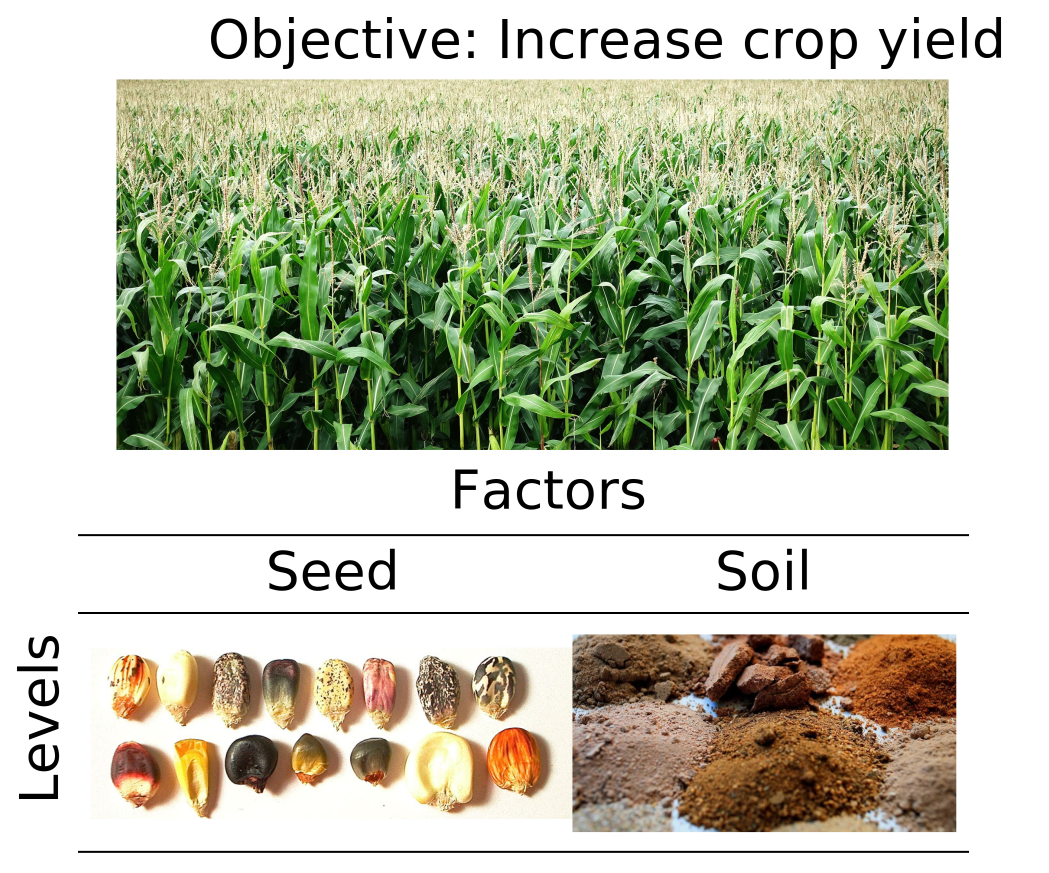
\includegraphics[width=.99\columnwidth]{../../../img/crop_yield_doe_example.pdf}
\end{center}
\end{column}
\begin{column}{0.45\columnwidth}
\begin{block}{Testing all combinations is \alert{inviable}}
\begin{block}{Which combinations to test?}
\begin{itemize}
\item ED provides a selection method
\item \colorbox{Highlight}{\alert{Parsimony}: decreases experiments}
\end{itemize}
\end{block}

\begin{block}{Which is the best combination?}
\begin{itemize}
\item ED provides an analysis method
\item \colorbox{Highlight}{\alert{Transparency}: uses statistical tests}
\end{itemize}
\end{block}
\end{block}
\end{column}
\end{columns}
\end{frame}

\begin{frame}[label={sec:org9ce9a09}]{Experimental Design}
\begin{columns}
\begin{column}{0.5\columnwidth}
\begin{block}{Terminology}
\begin{itemize}
\item Factors: program parameters
\item Levels: possible factor values
\item Experiment: setting each factor to a level
\item Design: a selection of experiments to run
\item \uncover<2>{Performance model: guides selection}
\end{itemize}

\begin{block}{Analyzing Results Enables:}
\begin{itemize}
\item Identifying \alert{significant factors}
\item Finding \alert{candidates} for further exploration
\item Investigating possible \alert{models}
\end{itemize}
\end{block}
\end{block}
\end{column}

\begin{column}{0.5\columnwidth}
\begin{block}{Example}
\vspace{-.2cm}
\begin{center}

A minimal screening design for \(7\) 2-level factors:

\end{center}
\vspace{-.2cm}

\only<1>{
\begin{table}[]
    \centering
    \begin{tabular}{@{\kern\tabcolsep}cccccccc@{\kern\tabcolsep}}
        \toprule
        Run & A & B & C & D & E & F & G \\ \midrule
        \cellcolor{gray!18}1 & \cellcolor{green!25}1 & \cellcolor{red!25}-1 & \cellcolor{green!25}1 & \cellcolor{red!25}-1 & \cellcolor{red!25}-1 & \cellcolor{green!25}1 & \cellcolor{green!25}1 \\
        \cellcolor{gray!18}2 & \cellcolor{green!25}1 & \cellcolor{green!25}1 & \cellcolor{green!25}1 & \cellcolor{red!25}-1 & \cellcolor{green!25}1 & \cellcolor{red!25}-1 & \cellcolor{red!25}-1 \\
        \cellcolor{gray!18}3 & \cellcolor{red!25}-1 & \cellcolor{green!25}1 & \cellcolor{red!25}-1 & \cellcolor{red!25}-1 & \cellcolor{green!25}1 & \cellcolor{green!25}1 & \cellcolor{green!25}1 \\
        \cellcolor{gray!18}4 & \cellcolor{red!25}-1 & \cellcolor{green!25}1 & \cellcolor{green!25}1 & \cellcolor{green!25}1 & \cellcolor{red!25}-1 & \cellcolor{green!25}1 & \cellcolor{red!25}-1 \\
        \cellcolor{gray!18}5 & \cellcolor{green!25}1 & \cellcolor{red!25}-1 & \cellcolor{red!25}-1 & \cellcolor{green!25}1 & \cellcolor{green!25}1 & \cellcolor{green!25}1 & \cellcolor{red!25}-1 \\
        \cellcolor{gray!18}6 & \cellcolor{green!25}1 & \cellcolor{green!25}1 & \cellcolor{red!25}-1 & \cellcolor{green!25}1 & \cellcolor{red!25}-1 & \cellcolor{red!25}-1 & \cellcolor{green!25}1 \\
        \cellcolor{gray!18}7 & \cellcolor{red!25}-1 & \cellcolor{red!25}-1 & \cellcolor{green!25}1 & \cellcolor{green!25}1 & \cellcolor{green!25}1 & \cellcolor{red!25}-1 & \cellcolor{green!25}1 \\
        \cellcolor{gray!18}8 & \cellcolor{red!25}-1 & \cellcolor{red!25}-1 & \cellcolor{red!25}-1 & \cellcolor{red!25}-1 & \cellcolor{red!25}-1 & \cellcolor{red!25}-1 & \cellcolor{red!25}-1  \\ \bottomrule
    \end{tabular}
\end{table}

}
\only<2>{
\begin{table}[]
    \centering
    \begin{tabular}{@{\kern\tabcolsep}ccccccccc@{\kern\tabcolsep}}
        \toprule
        Run & $\theta$ & A & B & C & D & E & F & G \\ \midrule
        \cellcolor{gray!18}1 & \cellcolor{blue!12}1 & \cellcolor{green!25}1 & \cellcolor{red!25}-1 & \cellcolor{green!25}1 & \cellcolor{red!25}-1 & \cellcolor{red!25}-1 & \cellcolor{green!25}1 & \cellcolor{green!25}1 \\
        \cellcolor{gray!18}2 & \cellcolor{blue!12}1 & \cellcolor{green!25}1 & \cellcolor{green!25}1 & \cellcolor{green!25}1 & \cellcolor{red!25}-1 & \cellcolor{green!25}1 & \cellcolor{red!25}-1 & \cellcolor{red!25}-1 \\
        \cellcolor{gray!18}3 & \cellcolor{blue!12}1 & \cellcolor{red!25}-1 & \cellcolor{green!25}1 & \cellcolor{red!25}-1 & \cellcolor{red!25}-1 & \cellcolor{green!25}1 & \cellcolor{green!25}1 & \cellcolor{green!25}1 \\
        \cellcolor{gray!18}4 & \cellcolor{blue!12}1 & \cellcolor{red!25}-1 & \cellcolor{green!25}1 & \cellcolor{green!25}1 & \cellcolor{green!25}1 & \cellcolor{red!25}-1 & \cellcolor{green!25}1 & \cellcolor{red!25}-1 \\
        \cellcolor{gray!18}5 & \cellcolor{blue!12}1 & \cellcolor{green!25}1 & \cellcolor{red!25}-1 & \cellcolor{red!25}-1 & \cellcolor{green!25}1 & \cellcolor{green!25}1 & \cellcolor{green!25}1 & \cellcolor{red!25}-1 \\
        \cellcolor{gray!18}6 & \cellcolor{blue!12}1 & \cellcolor{green!25}1 & \cellcolor{green!25}1 & \cellcolor{red!25}-1 & \cellcolor{green!25}1 & \cellcolor{red!25}-1 & \cellcolor{red!25}-1 & \cellcolor{green!25}1 \\
        \cellcolor{gray!18}7 & \cellcolor{blue!12}1 & \cellcolor{red!25}-1 & \cellcolor{red!25}-1 & \cellcolor{green!25}1 & \cellcolor{green!25}1 & \cellcolor{green!25}1 & \cellcolor{red!25}-1 & \cellcolor{green!25}1 \\
        \cellcolor{gray!18}8 & \cellcolor{blue!12}1 & \cellcolor{red!25}-1 & \cellcolor{red!25}-1 & \cellcolor{red!25}-1 & \cellcolor{red!25}-1 & \cellcolor{red!25}-1 & \cellcolor{red!25}-1 & \cellcolor{red!25}-1  \\ \bottomrule
    \end{tabular}
\end{table}

}
\vspace{-.2cm}

\uncover<2>{$$response = \theta{} + \alpha{}A + \beta{}B + \gamma{}C + \dots$$}
\end{block}
\end{column}
\end{columns}
\end{frame}

\begin{frame}[label={sec:org34b32f6}]{Search Heuristics: HLS for FPGAs}
\begin{columns}
\begin{column}{0.4\columnwidth}
\begin{block}{Autotuning HLS for FPGAs}
\begin{itemize}
\item CHStone benchmark
\item 141 factors, most with multiple levels
\item \alert{\(10^{128}\)} combinations
\item \alert{1\textasciitilde{}10min} to measure
\item \alert{Multiple objectives}
\item Search with meta-heuristics:
\begin{itemize}
\item Unstructured data hinders analysis
\end{itemize}
\end{itemize}
\end{block}
\end{column}
\begin{column}{0.6\columnwidth}
\begin{block}{Coverage of the Design Space}
\begin{center}
\includegraphics[width=.85\columnwidth]{../../../img/fpga_space.png}
\end{center}
\end{block}
\end{column}
\end{columns}
\end{frame}
\begin{frame}[label={sec:orga5144f1}]{Results: Targeting Performance}
\begin{columns}
\begin{column}{0.2\columnwidth}
\begin{block}{Metric Weights}
\begin{table}[htpb]
  \scriptsize
  \centering
  \begin{tabular}{@{}lcccc@{}}
    \toprule
    Metric & \textit{Performance} \\ \midrule
    \textit{LUT} & \cellcolor[HTML]{DD9583} Low \\
    \textit{Registers} & \cellcolor[HTML]{E3DBB3} Medium \\
    \textit{BRAMs} & \cellcolor[HTML]{DD9583} Low \\
    \textit{DSPs} & \cellcolor[HTML]{DD9583} Low \\
    \textit{FMax} & \cellcolor[HTML]{9B94B6} High \\
    \textit{Cycles} & \cellcolor[HTML]{DD9583} Low \\ \bottomrule
  \end{tabular}
\end{table}
\end{block}
\end{column}
\begin{column}{0.8\columnwidth}
\begin{block}{Improvements after 1.5h of Autotuning}
\begin{center}
\includegraphics[width=.9\linewidth]{../../../img/heatmap_default_stratixV_perf-eps-converted-to.pdf}
\end{center}

\begin{center}
\scriptsize{Autotuning high-level synthesis for \\ FPGAs using OpenTuner and LegUp (ReConFig 2017)}
\end{center}
\end{block}
\end{column}
\end{columns}
\end{frame}

\begin{frame}[label={sec:org26e8c02}]{Comparing Sampling Strategies: \(z = \theta + x + x^2 + y + y^2 + \varepsilon\)}
\begin{center}
\begin{center}
\includegraphics[width=.72\textwidth]{../../../img/sampling_comparison.pdf}
\end{center}
\end{center}
\end{frame}
\begin{frame}[label={sec:org2e7224a}]{A Experimental Design Approach to Autotuning}
\begin{center}
\begin{center}
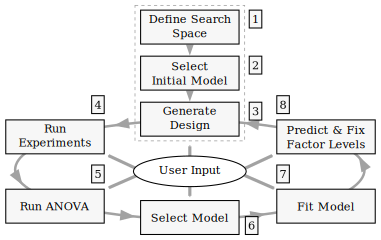
\includegraphics[width=.74\linewidth]{../../../img/doe_anova_strategy.pdf}
\end{center}

\vspace{-.2cm}
\end{center}

\begin{center}
\scriptsize{Autotuning under Tight Budget Constraints: \\ A Transparent Design of Experiments Approach (CCGRID 2019)}
\end{center}
\end{frame}
\begin{frame}[label={sec:orgfa13c78}]{GPU Laplacian Kernel: A Motivating Example}
\begin{columns}
\begin{column}{0.5\columnwidth}
\begin{block}{Search Problem}
\begin{itemize}
\item 7 parameters: 6 \alert{numerical}, 1 \alert{boolean}
\item Good starting performance model
\item Measured all 23120 configurations
\item Known \alert{global optimum}
\item Budget of \alert{125 points}
\end{itemize}
\end{block}
\end{column}

\begin{column}{0.5\columnwidth}
\begin{block}{Initial Model}
\footnotesize
\begin{align*}
cost = & \; y\_component\_number + 1 / y\_component\_number \; + \\
& \; vector\_length + lws\_y + 1 / lws\_y \; + \\
& \; load\_overlap + temporary\_size \; + \\
& \; elements\_number + 1 / elements\_number \; + \\
& \; threads\_number + 1 / threads\_number
\end{align*}
\normalsize
\end{block}
\end{column}
\end{columns}

\vspace{-.3cm}

\uncover<2>{
\begin{center}
  \colorbox{Highlight}{\parbox[c]{0.72\textwidth}{\centering We were  always close to
        the \alert{optimum} and used \alert{half of the budget}}}
\end{center}
}

\vspace{-.3cm}

\begin{center}
\begin{center}
\includegraphics[width=\columnwidth]{../../../img/comparison_histogram.pdf}
\end{center}
\end{center}
\end{frame}
\begin{frame}[label={sec:org702d255},fragile]{SPAPT: Search Problems in Automatic Performance Tuning}
 \begin{columns}
\begin{column}{0.41\columnwidth}
\begin{block}{Search Problem}
\begin{itemize}
\item \alert{Orio}: source code transformation
\item Baseline: \texttt{gcc -O3}, no transformations
\item Random sampling (\alert{RS}) vs. D-Optimal approach (\alert{DLMT})
\item 10 repetitions: measure \alert{speedup} and \alert{time-to-solution}
\item Out of 16 kernels:
\begin{itemize}
\item 3 with small impact
\item 6 with similar performance gains
\item \colorbox{Highlight}{7 with \alert{gains found faster}}
\end{itemize}
\end{itemize}
\end{block}
\end{column}
\begin{column}{0.59\columnwidth}
\begin{block}{Search Space}
\vspace{-0.4cm}

\begin{center}
\begin{table}[t]
\label{tab:spapt_apps}
\centering
\scriptsize
\begin{tabular}{llll}
\toprule
Kernel & Operation & Factors & Size\\
\midrule
\texttt{atax} & Matrix transp. \& vector mult. & 18 & \(2.6 \times 10^{16}\)\\
\texttt{dgemv3} & Scalar, vector \& matrix mult. & 49 & \(3.8 \times 10^{36}\)\\
\texttt{gemver} & Vector mult. \& matrix add. & 24 & \(2.6 \times 10^{22}\)\\
\texttt{gesummv} & Scalar, vector, \& matrix mult. & 11 & \(5.3 \times 10^{9}\)\\
\texttt{hessian} & Hessian computation & 9 & \(3.7 \times 10^{7}\)\\
\texttt{mm} & Matrix multiplication & 13 & \(1.2 \times 10^{12}\)\\
\texttt{mvt} & Matrix vector product \& transp. & 12 & \(1.1 \times 10^{9}\)\\
\texttt{tensor} & Tensor matrix mult. & 20 & \(1.2 \times 10^{19}\)\\
\texttt{trmm} & Triangular matrix operations & 25 & \(3.7 \times 10^{23}\)\\
\texttt{bicg} & Subkernel of BiCGStab & 13 & \(3.2 \times 10^{11}\)\\
\texttt{lu} & LU decomposition & 14 & \(9.6 \times 10^{12}\)\\
\texttt{adi} & Matrix sub., mult., \& div. & 20 & \(6.0 \times 10^{15}\)\\
\texttt{jacobi} & 1-D Jacobi computation & 11 & \(5.3 \times 10^{9}\)\\
\texttt{seidel} & Matrix factorization & 15 & \(1.3 \times 10^{14}\)\\
\texttt{stencil3d} & 3-D stencil computation & 29 & \(9.7 \times 10^{27}\)\\
\texttt{correlation} & Correlation computation & 21 & \(4.5 \times 10^{17}\)\\
\bottomrule
\end{tabular}
\end{table}

\scriptsize{Balaprakash P, Wild SM, Norris B. SPAPT: Search problems in automatic performance tuning. Procedia Comp. Sci. 2012 Jan 1;9:1959-68.}
\end{center}
\end{block}
\end{column}
\end{columns}
\end{frame}

\begin{frame}[label={sec:org5718037}]{SPAPT: Search Problems in Automatic Performance Tuning}
\begin{center}
\begin{center}
\includegraphics[width=\linewidth]{../../../img/iteration_best_comparison.pdf}
\end{center}
\end{center}
\end{frame}
\begin{frame}[label={sec:orga0385f3}]{SPAPT: Search Problems in Automatic Performance Tuning}
\begin{center}
\includegraphics[width=\columnwidth]{../../../img/split_histograms.pdf}
\end{center}
\end{frame}
\begin{frame}[label={sec:org058b84f}]{SPAPT: Looking for Structure in \emph{bicgkernel}}
\begin{columns}
\begin{column}{0.5\columnwidth}
\begin{block}{ED Methods for \emph{bicgkernel}}
\alert{Consistently} fixes parameters and levels:
\begin{itemize}
\item Quickly identifies \alert{global} structure
\item Restricts to better sub-regions
\end{itemize}

Further exploration:
\begin{itemize}
\item Certain strong effects \alert{``mask''} others
\item Improving starting model:
\begin{itemize}
\item Cubic terms were not significant
\end{itemize}
\end{itemize}
\end{block}
\end{column}
\begin{column}{0.5\columnwidth}
\only<1>{
\begin{center}
\includegraphics[width=\columnwidth]{../../../img/bicgkernel_factors.pdf}
\end{center}
}
\only<2>{
\begin{center}
\includegraphics[width=\columnwidth]{../../../img/bicgkernel_updated.pdf}
\end{center}
}
\end{column}
\end{columns}
\end{frame}
\begin{frame}[label={sec:org43744f4}]{Laplacian and SPAPT kernels Experiments}
With these initial experiments, we showed that:

\begin{columns}
\begin{column}{0.5\columnwidth}
\begin{itemize}
\item Exploiting \alert{global search space structure} helps finding good configurations
fast
\end{itemize}
\end{column}
\begin{column}{0.5\columnwidth}
\begin{itemize}
\item The ED approach is parsimonious, transparent, and \alert{effective} for autotuning
\end{itemize}
\end{column}
\end{columns}
\vspace{0.5cm}
In order  to identify  and exploit \alert{local  structures}, we  need:

\begin{itemize}
\item More \alert{modeling ``flexibility''}
\item \alert{Domain knowledge}
\end{itemize}

\begin{block}{Efforts for Reproducibility}
\begin{center}
\colorbox{Highlight}{\parbox[c]{0.54\textwidth}{\centering \alert{Source code} \& \alert{data} at github.com/phrb/ccgrid19}}
\end{center}
\end{block}
\end{frame}


\begin{frame}[label={sec:org4e9112c}]{Autotuning DNN Quantization}
\begin{center}
\includegraphics[width=.7\columnwidth]{../../../img/haq_quantization_II.pdf}
\end{center}

\begin{center}
\scriptsize{HAQ: Hardware-Aware Automated Quantization with Mixed Precision (CV 2018)}
\end{center}
\end{frame}
\end{document}
